\chapter{Implementation}
\label{chap:Implementation}

This chapter details the design process of the swarm system, and the approach used when tackling the problem of multi-agent interactions.

Firstly, an outline of the problem representation is shown and then the structure and reasoning behind the software implementation.

\section{Design}

As shown in section \ref{section: hardware}, the standard configuration of the e-puck has all of the required capabilities to implement swarming behaviour.

\subsection{Simulation Setup}

Firstly, a new project was created in Webots.

This defined the virtual operating environment and the number of robots in the world, as well as the world parameters. Shown in Figures \ref{fig:world-param} and \ref{fig:arena-param} are the parameters used for the simulation, all other parameters were kept as the default.

The simulation consisted of a bounded, rectangular arena of size 3 metres by 3 metres. Within this arena, there are two wooden boxes (one of size 0.2m x 0.2m x 0.2m and the other of size 0.5m x 0.5m x 0.5m) and a hollow cylinder (of height 0.3m, radius 0.2m and thickness 0.1m). In the setup shown, only 9 e-pucks are utilised, placed in random locations around the arena, see Figure \ref{fig:arena}.

\tabulinesep = 1mm
\begin{figure}[!h]
	\centering
	\begin{minipage}{.45\textwidth}
		\centering
		\begin{tabu} to .75\textwidth { | X[l] | X[c] | }
			\hline
			Basic time step & 32ms \\
			\hline
			Frames per second & 60 \\
			\hline
			North direction & -10m \\
			\hline
			Objects & 3 \\
			\hline
			e-pucks & 9 \\
			\hline
		\end{tabu}
	\caption{World parameters} 	% \caption IS ALWAYS FIRST
	\label{fig:world-param} 	% \label IS ALWAYS SECOND
	\end{minipage}
	\begin{minipage}{.45\textwidth}
		\centering
		\begin{tabu} to .75\textwidth { | X[l] | X[c] | }
			\hline
			Length (x) & 3 metres \\
			\hline
			Breadth (y) & 3 metres \\
			\hline
			Wall thickness & 0.01 metres \\
			\hline
			Wall height & 0.1 metres \\
			\hline
		\end{tabu}
	\caption{Arena parameters} 	% \caption IS ALWAYS FIRST
	\label{fig:arena-param} 	% \label IS ALWAYS SECOND
	\end{minipage}
\end{figure}

\begin{figure}[h]
		\centering
		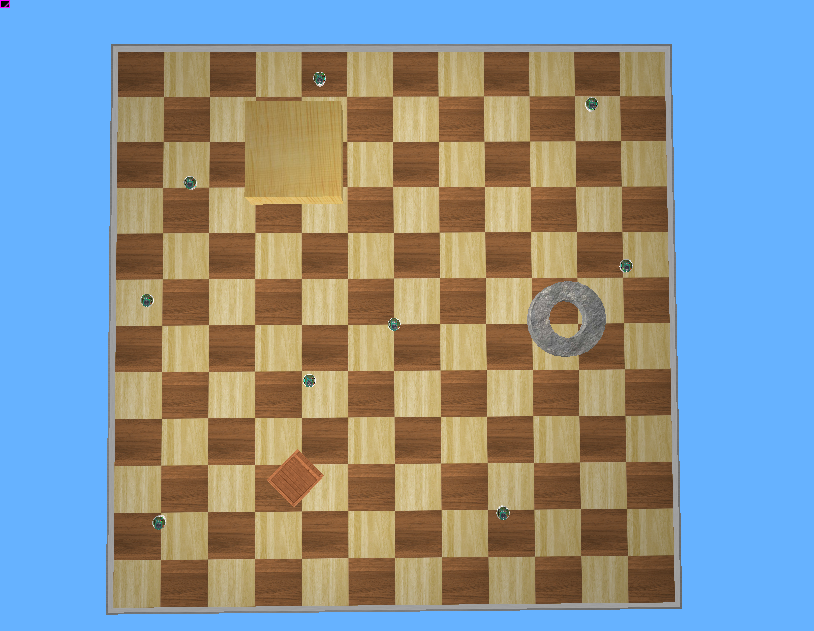
\includegraphics[width=.6\linewidth]{top-down-simulation}
		\captionof{figure}{Arena}
		\label{fig:arena}
\end{figure}

\begin{figure}[!h]
	\centering
	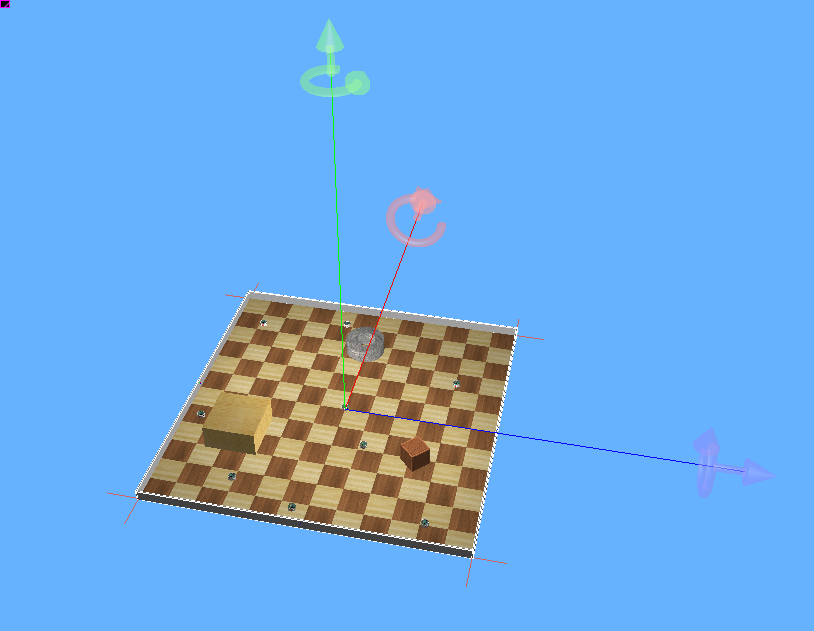
\includegraphics[width=.6\linewidth]{sideways}
	\captionsetup{width=.7\textwidth}
	\captionof{figure}{Arrows denote the positive world axes directions}
	\label{fig:axes}
\end{figure}

Figure \ref{fig:axes} shows the positive directions of the x, y and z axes. Red denotes positive x, green denotes positive y, blue denotes positive z. Hence the north direction has been set to (0, 0, -10). \newline

The arena was setup in the manner shown in Figure \ref{fig:arena} after careful consideration of evaluation parameters:-

\begin{enumerate}
	\item Obstacles of various shapes and sizes tests the ability of the swarm and its agents to avoid obstacles.
	\item The positioning of the large box and cylinder creates narrow corridors against the arena walls and this tests the swarm's ability to navigate confined spaces.
	\item Objects will block line of sight (and therefore sensing) to other robots and this tests the ability of the swarm to form splinter groups.
	\item Open spaces will test the ability of these splinter groups to amalgamate and form a singular flock.
\end{enumerate}

Furthermore, this project differs from other demonstrations of swarm behaviour due to the fact that there is no overall destination for the flock to head towards (such as a user-defined point). Any resulting shapes or patterns formed by the swarm are entirely emergent.

\subsection{e-puck Model Modifications}
\label{subsection:mod-desc}

Though the model provided by Webots was sufficient for this project's intended aplication, some modifications were made to simplify the simulation and aid in the collecting of experimental data.

As stated in subsection \ref{subsection:hardware-desc}, the e-puck is capable of robot-robot communication utilising the IR sensors as receivers and emitters. However, the implemented sensors (Fig. \ref{fig:epuck-sensors}) are purely proximity and light sensors and does not detect IR light from other robots, only the reflection of its own signal. Thus, the simulated e-pucks are incapable of using exactly the same method of IR communication as real e-pucks.

This problem can be overcome through the use of Webots' supplied ``Emitter'' and ``Receiver'' nodes. These are additional modules that can be added to a model and simulate a method of communication. In this case the desired method of communication is through the medium of infra-red, though radio is possible.

One solution was to add an emitter and receiver at the positions of each proximity sensor. The emitter and receiver can then be limited to match the range and aperture of the IR sensors. This would closely emulate the way a real e-puck would use the sensors to communicate. However, this would be computationally expensive to execute, as the simulator would have to process at worst eight incoming/outgoing messages per e-puck and over a large swarm could cause issues with memory and performance.

A better solution was implemented. Instead of eight emitter/receiver pairs, only one is utilised, placed on top of the centre of the robot. However, this emitter/receiver has a wide aperture of 360\textdegree. In this manner, the simulated robot can communicate with any neighbouring flockmates in a similar way to real e-puck, while significantly reducing the computational overhead of the simulator.

Another modification made was the addition of a GPS unit to each e-puck. This is not utilised during the course of exhibiting flocking behaviour, rather it is added as an experimental tool to collect data on the trajectories of every e-puck in the world.

\section{Code Implementation}

The approach taken to implementing the desired swarming behaviour can be divided into two processes: defining the low level dependencies of the system, and then defining the high level operations.

A full code listing can be found in Appendix TODO.

\begin{comment}
\begin{lstlisting}
for (int i=0; i<iterations;i++)
{
do something
}
\end{lstlisting}
\end{comment}


\subsection{Libraries and dependencies}

In order to keep system complexity as low as possible, the use of any external C++ libraries were minimised. In this project, only the default Webots function library and the C++ standard library were utilised. This also aids in keeping program compatibility across different computers and operating systems.

The use of the \textit{libircom} library for infra-red communication using the proximity sensors was investigated at the early stages of this project, though this was eschewed due to the problems outlined in section \ref{subsection:mod-desc}.
\clearpage

\subsection{Algorithm Heirarchy}

The algorithm can be split up into three main processes: receive data from the environment and other agents (proximity sensors and messages), process the received data and decide on the next course of action, execute the next course of action. 

Figure \ref{fig:flow-1} shows a highly abstracted procedure of the robot controller. Subsequent flow charts will detail the lower level processes within each abstracted process.

\subsubsection{Overall procedure}

\tikzstyle{decision} = [diamond, draw, fill=green!20, 
text width=3cm, text badly centered, node distance=3cm, inner sep=0pt]
\tikzstyle{block} = [rectangle, draw, fill=blue!20, 
text width=4cm, text centered, rounded corners, minimum height=4em]
\tikzstyle{line} = [draw, -latex']
\tikzstyle{cloud} = [draw, ellipse,fill=red!20, node distance=3cm,
minimum height=2em]
\tikzstyle{arrow} = [thick,->,>=stealth]

\begin{figure}[h]
	\centering
	\begin{tikzpicture}[node distance = 3cm]
	\node [cloud] (start) {Start};
	\node [block, below of=start] (getData) {Obtain data from the environment};
	\node [block, below of=getData] (process) {Decide on next action};
	\node [block, below of=process] (actuate) {Act on processed data};
	\node [decision, below of=actuate] (quit) {Stop condition met?} ;
	\node [cloud, below of=quit, node distance=3cm] (stop) {stop};
	% Draw edges
	\draw [arrow] (start) -- (getData);
	\draw [arrow] (getData) -- (process);
	\draw [arrow] (process) -- (actuate);
	\draw [arrow] (actuate) -- (quit);
	\draw [arrow] (quit) -- node[anchor=east] {yes}(stop) ;
	\draw [arrow] (quit.east) -- ++(1cm,0) node[above] {no} -- ++(1cm,0) |- (getData.east);
	%\path [line] (decide) -| node [near start] {yes} (update);
	%\path [line] (update) |- (stop);
	%\path [line] (decide) -- node {no}(stop);
	\end{tikzpicture}
	\captionof{figure}{Simplified algorithm procedure}
	\label{fig:flow-1}
\end{figure}

\clearpage

\subsubsection{Obtaining data}

\begin{figure}[h]
	\centering
	\begin{tikzpicture}[node distance = 3cm]
	\node [cloud] (start) {Start};
	\node [block, below of=start] (getData) {Get raw messages from the IR receiver};
	\node [block, below of=getData] (process) {Process message data};
	\node [block, below of=process] (compass) {Poll compass for bearing};
	\node [block, below of=compass] (distanceCheck) {Poll proximity sensors for obstacles};
	\node [cloud, below of=distanceCheck] (continue) {cont'd};
	% Draw edges
	\draw [arrow] (start) -- (getData);
	\draw [arrow] (getData) -- (process);
	\draw [arrow] (process) -- (compass);
	\draw [arrow] (compass) -- (distanceCheck);
	\draw [arrow] (distanceCheck) -- (continue);
	\end{tikzpicture}
	\captionof{figure}{First process}
	\label{fig:flow-2}
\end{figure}

\clearpage


\begin{lstlisting}[language=C++, caption={Message protocol},label={lst:mess-receive}]
void Swarm::getReceiverData() {
	Receiver *copy = (Receiver *)malloc(sizeof(Receiver));
	myData.orientationString = {};
	robots = roundNum((receiver->getQueueLength() + 1) / 2);
	for (int i = 0; i < 100; i++) {
		signalStrength[i] = 0;
	}
	for (int k = 0; k < receiver->getQueueLength(); k++) {
		data = (char *)receiver->getData();
		signalStrength[k] = (double)receiver->getSignalStrength();
		for (int n = 0; n < 3; n++) {
			emitterDirection[k][n] = 
										receiver->getEmitterDirection()[n];
		}
		memcpy(copy, data, sizeof(Receiver));
		myData.orientationString[k] = (char *)copy;
		receiver->nextPacket();
	}
}
\end{lstlisting}

Listing \ref{lst:mess-receive} shows the procedure used to convert a raw message from another robot, into a string type. This function also processes a number of global variables: the number of detected robots in the neighbourhood, the signal strength (and thus distance) of the message signal and the direction of the message signal. Having a euclidean distance and an angle allows the robot to obtain a vector to the message origin.

\clearpage

\begin{lstlisting}[language=C++, caption={Message processing},label={lst:mess-pro}]
void Swarm::processReceiverData(std::array<std::string, ARRAY_SIZE> data) {
	myData.received = false;
	for (unsigned int i = 0; i < ARRAY_SIZE; i++) {
		myData.orientationDouble[i] = 0;
	}
	try {
		std::regex re("[*0-9*.*0-9*]+");
		for (int i = 0; i < robots; i++) {
			std::sregex_iterator next(data[i].begin(), data[i].end(), re);
			std::sregex_iterator end;
			while (next != end) {
				std::smatch match = *next;
				std::string match1 = match.str();
				myData.orientationDouble[i] = atoi(match1.c_str());
				if (myData.orientationDouble[i] >= 352) {
				myData.orientationDouble[i] = 0;
				}
				next++;
				if (next == end) {
					myData.received = true;
				}
			}
		}
	} catch (std::regex_error &e) {}
}
\end{lstlisting}

Listing \ref{lst:mess-pro} details the method by which a received message of type string is processed. This was achieved by iterating through an array containing the messages from every robot and using a regular expression to parse these strings. The regular expression, in this case, searches for a decimal number with trailing digits. If a match is detected, the number is converted from a string type into a double type and saved in a global variable (line 14).

\clearpage

\begin{lstlisting}[language=C++, caption={Getting orientation data},label={lst:compass-poll}]
void Swarm::saveCompassValues() {
	const double *compassVal = compass->getValues();
	for (int i = 0; i < 3; i++) {
		currentOrientation[i] = compassVal[i];
	}
}
\end{lstlisting}

Listing \ref{lst:compass-poll} shows how the robot can access the data from the compass module in order to obtain its orientation in the world. The data returned from the compass module is a three dimensional vector toward the north point within the simulation.

\begin{lstlisting}[language=C++, caption={Getting proximity information},label={lst:prox}]
void Swarm::distanceCheck() {
	for (int i = 0; i < 8; i++) {
		ps_values[i] = checkDistanceSensor(i);
	}
	right_obstacle = (ps_values[0] > PS_THRESHOLD) || (ps_values[1] > PS_THRESHOLD) || (ps_values[2] > PS_THRESHOLD);
	left_obstacle = (ps_values[5] > PS_THRESHOLD) || (ps_values[6] > PS_THRESHOLD) || (ps_values[7] > PS_THRESHOLD);
	front_obstacle = (ps_values[0] > PS_THRESHOLD) & (ps_values[7] > PS_THRESHOLD);
	back_obstacle = (ps_values[3] > PS_THRESHOLD) & (ps_values[4] > PS_THRESHOLD);
}
\end{lstlisting}

Listing \ref{lst:prox} demonstrates how the robot can access the data from its circumferential proximity sensors. In this case, the sensors are discretized into ranges, depending on the position of the sensor on the robot. If the value of a sensor within that range is above a certain user defined threshold, a boolean value is set.

\clearpage

\subsubsection{Decision and actuation}
\begin{figure}[!h]
	\centering
	\begin{tikzpicture}[node distance = 2.5cm,auto]
\node [cloud] (start) {Obtaining data};
\node [block, below of=start] (direction) {Obtain directions of detected robots};
\node [decision, below of=direction] (check1) {Other robots and no obstacles?};
\node [block, below of=check1, yshift = -1cm] (adjust) {Steer towards nearest neighbour};
\node [block, right of=adjust, xshift=3cm] (object) {Steer away from any object};
\node [decision, below of=adjust] (check2) {Robots $\geq$ 1?};
\node [block, below of=check2, yshift=-0.2cm] (range) {Change emitter range};
\node [block, below of=range] (send) {Send current orientation};
\node [decision, below of=send] (check3) {Stop key pressed?};
\node [cloud, right of=check3] (stop) {Stop};
% Draw edges
\draw [arrow] (start) -- (direction);
\draw [arrow] (direction) -- (check1);
\draw [arrow] (check1) -| node {no} (object);
\draw [arrow] (check1) -- node {yes} (adjust);
\draw [arrow] (adjust) -- (check2);
\draw [arrow] (object) |- (check2.north);
\draw [arrow] (check2) -- node {yes} (range);
\draw [arrow] (check2) -| ++(5cm,0) -- ++(0,-5.2cm) -- node {no} (send.east);
\draw [arrow] (range) -- (send);
\draw [arrow] (send) -- (check3);
\draw [arrow] (check3.east) -- node{yes} (stop);
\draw [arrow] (check3.west) -- node[above]{no} ++(-2cm,0) -- ++(0cm,20.2) -- (start);
	\end{tikzpicture}
	\captionof{figure}{Second and third process}
	\label{fig:flow-3}
\end{figure}

\begin{lstlisting}[language=C++, caption={Calculating target vector},label={lst:dir-vec}]
int index = std::distance(signalStrength, std::max_element(signalStrength, signalStrength + sizeof(signalStrength) / sizeof(double)));

std::array<double, 3> direction = {0, 0, 0};

if (robots > ALIGN_THRESHOLD) {
	for (int k = 0; k < 3; k++) {
		direction[k] = emitterDirection[index + 1][k];
	}
} else if (robots == 1) {
	for (int k = 0; k < 3; k++) {
		direction[k] = emitterDirection[index][k];
	}
}

double nearestNeighbour = computeVectorAngle(direction);
\end{lstlisting}

Listing \ref{lst:dir-vec} demonstrates the method by which the robot can determine the direction of the neighbour it should steer toward. This is achieved by returning the vector of its second nearest neighbour in the case that the number of robots detected is greater than a pre-defined value, or the nearest neighbour in the case that only one robot is detected.

\begin{lstlisting}[language=C++, caption={Action for next step},label={lst:fsm}]
if ((robots >= ALIGN_THRESHOLD) && (!left_obstacle) && (!right_obstacle) && signalStrength[index] < 10) {
	setLEDs(0);
	adjust(nearestNeighbour);
} else {
	setLEDs(1);
	objectDetection(1.0);
}
\end{lstlisting}

Listing \ref{lst:fsm} is a crucial step in the algorithm. This process defines the behaviour that the robot will exhibit at the next time step. If a certain condition is met (there are sufficient robots in the neighbourhood and no obstacles detected and the nearest neighbour is far way), the robot steers towards the direction calculated in Listing \ref{lst:dir-vec}. Else, the robot will exhibit obstacle avoidance. The parameter for \textit{objectDetection} (line 6) is simply a speed multiplier i.e. exhibit obstacle at 1.0*normal speed. In each case, the robot either switches its circumferential LEDs on or off and this aids the user in determining the state of the robot during simulation.

\begin{lstlisting}[language=C++, caption={Adjust heading},label={lst:adjust}]
void Swarm::adjust(double angle) {
	double left_speed = WHEEL_SPEED;
	double right_speed = WHEEL_SPEED;
	
	if (((angle > (360 - ALIGN_ERROR)) & (angle < 360)) | ((angle > 0) & (angle < ALIGN_ERROR))) {
		right_speed = left_speed = WHEEL_SPEED;
	} else if ((angle > 270) & (angle < (360 - ALIGN_ERROR))) {
		left_speed = (1 + (ALIGN_ERROR + angle - 360) / (90 - ALIGN_ERROR)) * WHEEL_SPEED;
		right_speed = WHEEL_SPEED;
	} else if ((angle >= 180) & (angle < 270)) {
		left_speed = ((angle - 270) / 90) * WHEEL_SPEED;
		right_speed = WHEEL_SPEED;
	} else if ((angle >= 90) & (angle < 180)) {
		right_speed = ((90 - angle) / (90)) * WHEEL_SPEED;
		left_speed = WHEEL_SPEED;
	} else if ((angle >= ALIGN_ERROR) & (angle < 90)) {
		right_speed = (1 - (angle - ALIGN_ERROR) / (90 - ALIGN_ERROR)) * WHEEL_SPEED;
		left_speed = WHEEL_SPEED;
	}
	
	if (left_speed > 1000) {
		left_speed = 1000;
	}
	
	if (right_speed > 1000) {
		right_speed = 1000;
	}
	
	move((int)left_speed, (int)right_speed);
}
\end{lstlisting}

Listing \ref{lst:adjust} details the method by which the robot adjusts its heading to steer toward a specified angle. 

Given an angle to steer toward, this function adjust the wheel speeds dynamically dependent on the magnitude of the error to a ``zero'' heading. For example, adjusting to a heading of 180\textdegree will result in a more pronounced speed difference versus adjusting to a heading infront of the robot.

\begin{figure}[h]
	\centering
	\begin{minipage}{.75\textwidth}
		\centering
		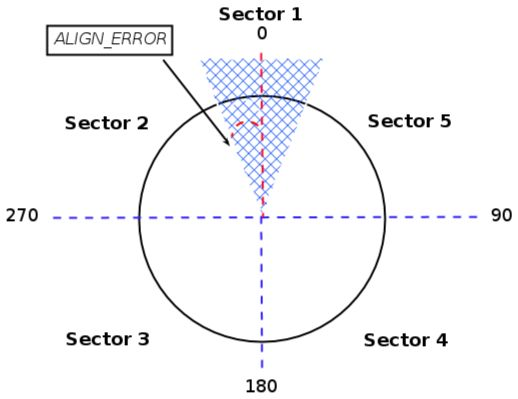
\includegraphics[width=1\linewidth]{sections_robot}
		\captionof{figure}{Sector discretizations}
		\label{fig:robot-sectors}
	\end{minipage}
\end{figure}

Shown in Figure \ref{fig:robot-sectors} are the sectors of the angle discretizations. It was necessary to apply an error value, \textit{ALIGN\_ERROR}, when determining a ``zero'' heading to prevent unwanted oscillations. The function determines which of these sectors the desired heading is located in and applies one of several velocity equations:-

\begin{enumerate}
	\item \textit{left wheel speed} = BASE\_WHEEL\_SPEED \newline
	\textit{right wheel speed} = BASE\_WHEEL\_SPEED
	
	\item \textit{left wheel speed} = \(1 + \dfrac{ANGLE\_ERROR + angle - 360}{90 - ANGLE\_ERROR} \times BASE\_WHEEL\_SPEED\) \newline
	\textit{right wheel speed} = BASE\_WHEEL\_SPEED
	
	\item \textit{left wheel speed} = \(\dfrac{angle - 270}{90} \times BASE\_WHEEL\_SPEED\) \newline
	\textit{right wheel speed} = BASE\_WHEEL\_SPEED
	
	\item \textit{left wheel speed} = BASE\_WHEEL\_SPEED  \newline
	\textit{right wheel speed} = \(\dfrac{90 - angle}{90} \times BASE\_WHEEL\_SPEED\)
	
	\item \textit{left wheel speed} = BASE\_WHEEL\_SPEED  \newline
	\textit{right wheel speed} = \(1 + \dfrac{ANGLE\_ERROR + angle - 360}{90 - ANGLE\_ERROR} \times BASE\_WHEEL\_SPEED\)
	
\end{enumerate}

\subsection{Low level}

It is essential that the low level operations are first constructed, before any implementation of the higher level behaviour is undertaken. 

This is because some of the higher level functions will rely on the lower level operations. For example, in order for a robot to move towards another robot, there are a host of underlying operations that will need to be performed before the physical actuation of the wheels begin.

Perhaps



\subsection{High level}

